% !TEX program = xelatex
% ¡Recuerda compilar con XeLaTeX o LuaLaTeX!
\documentclass{article}

% --- Cargar nuestro fichero de estilo ---
% Se asume que paper_style.sty está disponible o se usan paquetes estándar.
\usepackage{paper_style}

% --- PAQUETES PARA EL CONTENIDO DEL DOCUMENTO ---
\usepackage{graphicx}
\usepackage{subcaption}
\usepackage{amsmath}
\usepackage{booktabs}
\usepackage{geometry}
\usepackage{hyperref}
\usepackage{enumitem}
\usepackage{float}



% --- Información del Paper ---
\title{Informe: \\ Introducción a la Consola de Administración de AWS}
\author{
	Jordi Blasco Lozano \\
	\small Infraestructuras y Servicios Cloud \\
	\small Universidad de Alicante
}
\date{\today}

% --- Comienzo del Documento ---
\begin{document}
	
	\maketitle

	\begin{abstract}
	\noindent 
	\end{abstract}

	\tableofcontents

	\newpage

	\section{Creación de la instancia base}

		Para poder tener la pagina web desplegada debemos de iniciar la primera instancia. Esta primera instancia vendrá de una imagen limpia de Amazon Linux. Nos conectaremos mediante ssh a la instancia para instalar httpd y poder cargar el html copiando con nano.

	\subsection{Configuración de red}

		\noindent Para poder acceder a nuestro servidor mediante una url debemos de configurar la instancia de forma que permita accesos http y https. Esto lo podemos hacer desde el panel de configuración de ``lanzar una instancia''. 



	\begin{figure}[H]
	\centering
	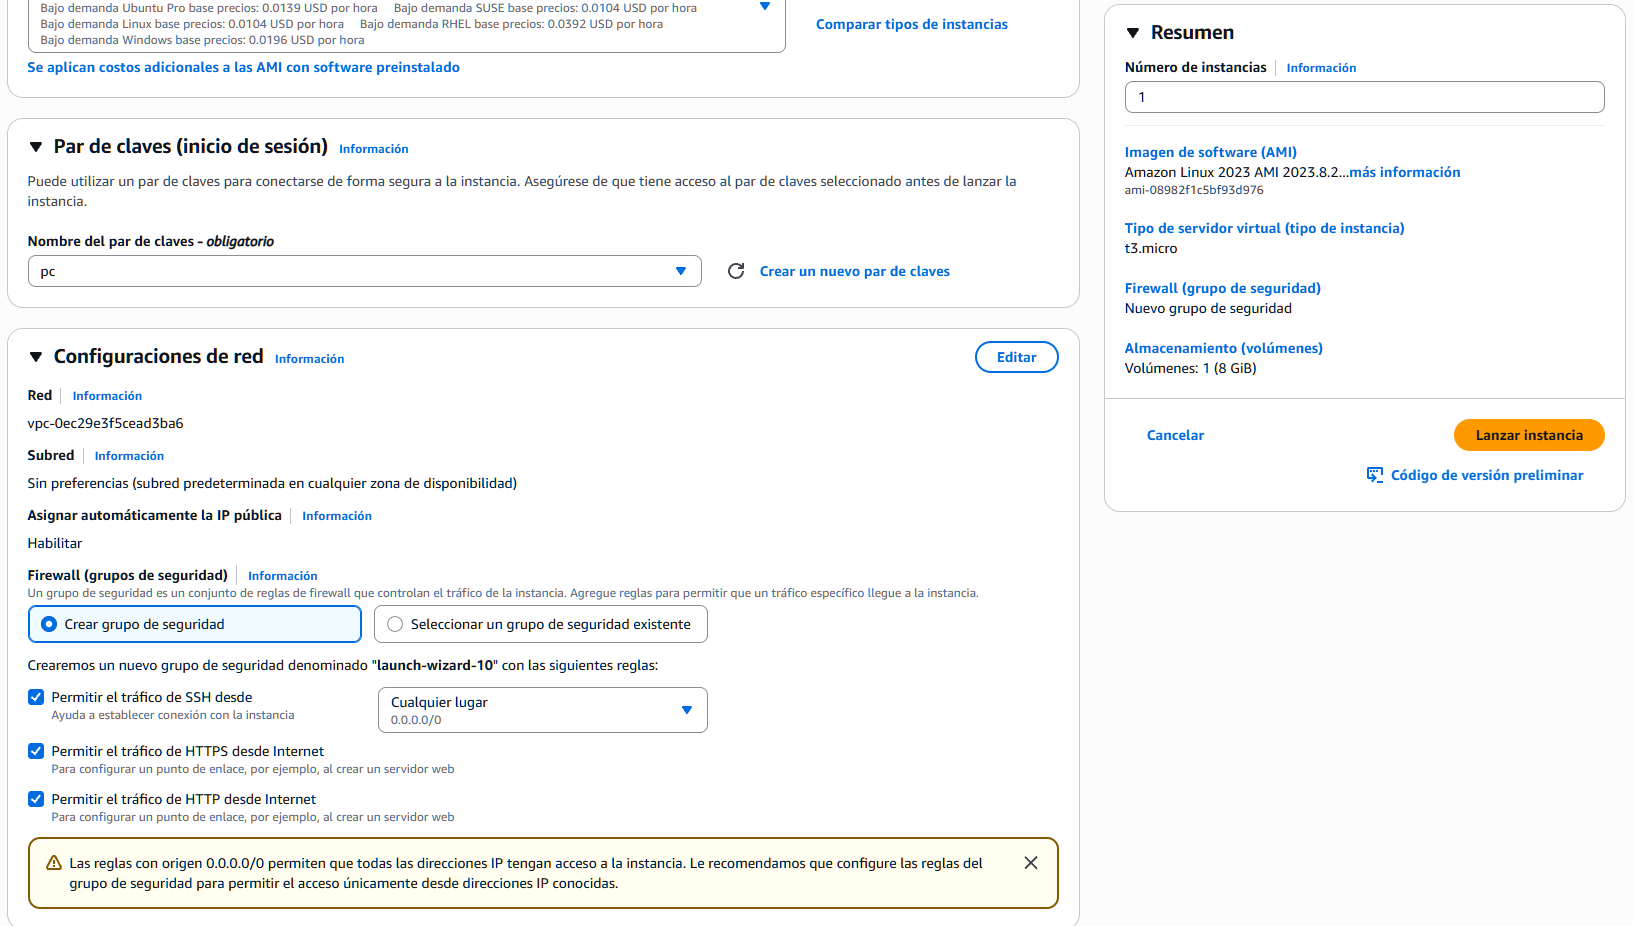
\includegraphics[width=0.95\textwidth]{configuracion_IC2.png}
	\caption{panel de lanzar una instancia}
	\end{figure}

	\begin{figure}[H]
	\centering
	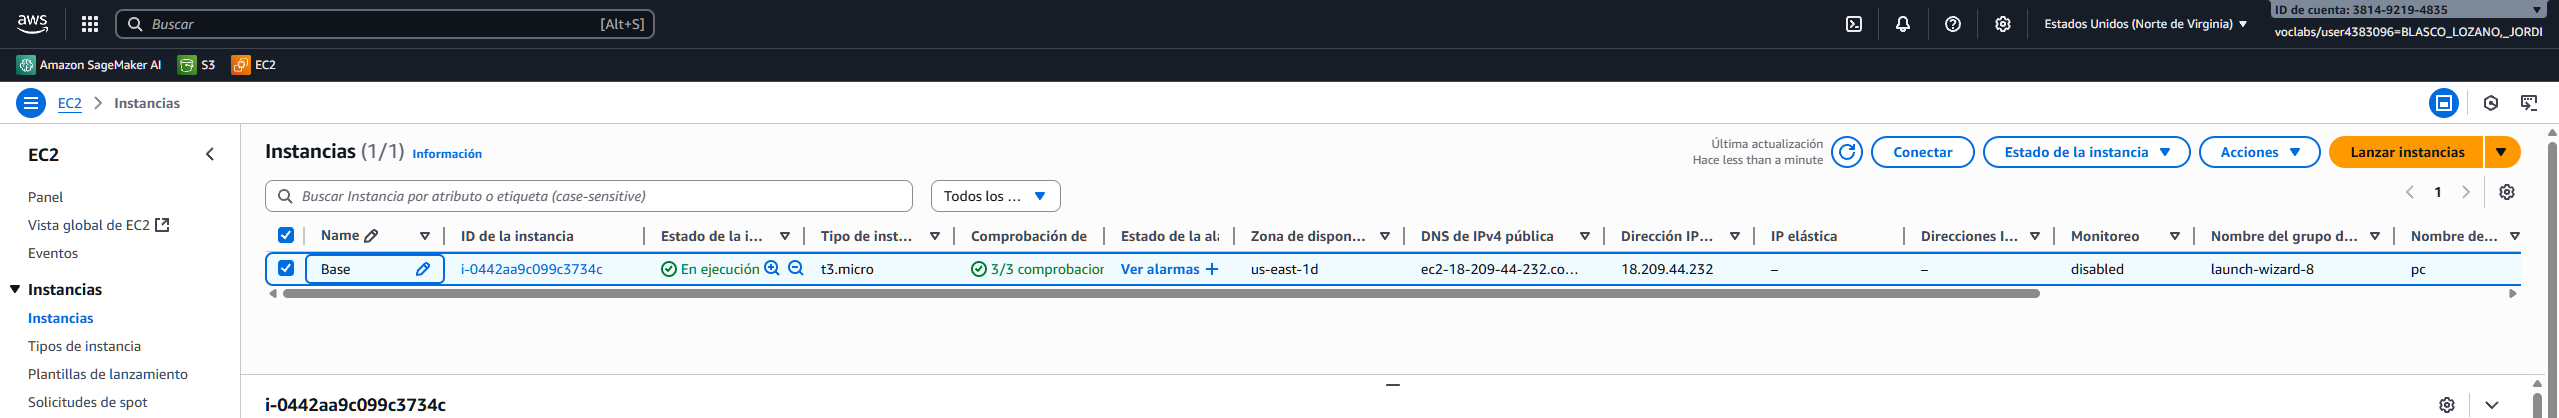
\includegraphics[width=0.95\textwidth]{pestanya_instancias.png}
	\caption{Panel de instancias}
	\end{figure}
\newpage

	\subsection{Instalación de dependencias}

		Una vez tengamos la instancia creada deberemos de conectarnos a ella por ssh. Cuando estemos dentro de la instancia instalaremos httpd mediante el comando sudo yum install httpd. httpd es un servidor web Apache que utilizaremos para desplegar nuestro index.html.


\begin{lstlisting}[style=consola, language=bash, caption={Terminal, dependencias}]
   ,     #_
   ~\_  ####_        Amazon Linux 2023
  ~~  \_#####\
  ~~     \###|
  ~~       \#/ ___   https://aws.amazon.com/linux/amazon-linux-2023
   ~~       V~' '->
    ~~~         /
      ~~._.   _/
         _/ _/
       _/m/'
[ec2-user@ip-172-31-30-24 ~]$ sudo yum install httpd
Amazon Linux 2023 Kernel Livepatch repository                                           177 kB/s |  23 kB     00:00
Dependencies resolved.
==================================================================================
 Package                         Architecture       Version                               Repository               Size
==================================================================================
Installing:
 httpd                           x86_64             2.4.65-1.amzn2023.0.1                 amazonlinux              47 k
Installing dependencies:
...

Transaction Summary
==================================================================================
Install  12 Packages
...

Complete!
[ec2-user@ip-172-31-30-24 ~]$

\end{lstlisting}

\subsection{Archivo index.html}

	La pagina web que queremos desplegar aun no se encuentra dentro de la instancia. Para que Apache cargue este archivo debemos de hacer dos cosas, la primera es navegar hasta /var/www/html, que es donde httpd debe de encontrar el archivo index.html; la segunda es crear este archivo y usar nano para pegarlo. Posteriormente si no estamos seguros de haber usado nano bien podemos hacer cut para mostrar que se haya escrito correctamente. Aquí se muestra como lo he realizado.


\begin{lstlisting}[style=consola, language=bash, caption={Terminal, index.html}]
[ec2-user@ip-172-31-30-24 ~]$ cd /var/www/html
[ec2-user@ip-172-31-30-24 html]$ sudo nano index.html
[ec2-user@ip-172-31-30-24 html]$ cat /var/www/html/index.html
<!DOCTYPE html>
<html lang="es">
<head>
    <meta charset="UTF-8">
...
\end{lstlisting}
\newpage
\subsection{Comandos de start y habilitación}

	Después de haber creado el archivo html debemoos de utilizar los comandos de systemctl para iniciar y habilitar el servidor Apache. Finalmente podemos comprobar si esta habilitado usando el comando para status de esta forma. 

\begin{lstlisting}[style=consola, language=bash, caption={Terminal, systemctl}]
[ec2-user@ip-172-31-30-24 html]$ sudo systemctl start httpd
[ec2-user@ip-172-31-30-24 html]$ sudo systemctl enable httpd
Created symlink /etc/systemd/system/multi-user.target.wants/httpd.service → /usr/lib/systemd/system/httpd.service.
[ec2-user@ip-172-31-30-24 html]$ sudo systemctl status httpd
● httpd.service - The Apache HTTP Server
     Loaded: loaded (/usr/lib/systemd/system/httpd.service; enabled; preset: disabled)
     Active: active (running) since Wed 2025-09-17 17:20:09 UTC; 2min 11s ago
       Docs: man:httpd.service(8)
   Main PID: 27040 (httpd)
     Status: "Total requests: 0; Idle/Busy workers 100/0;Requests/sec: 0; Bytes served/sec:   0 B/sec"
      Tasks: 177 (limit: 1057)
     Memory: 13.3M
        CPU: 180ms
     CGroup: /system.slice/httpd.service
             ├─27040 /usr/sbin/httpd -DFOREGROUND
             ├─27041 /usr/sbin/httpd -DFOREGROUND
             ├─27042 /usr/sbin/httpd -DFOREGROUND
             ├─27043 /usr/sbin/httpd -DFOREGROUND
             └─27044 /usr/sbin/httpd -DFOREGROUND

Sep 17 17:20:09 ip-172-31-30-24.ec2.internal systemd[1]: Starting httpd.service - The Apache HTTP Server...
Sep 17 17:20:09 ip-172-31-30-24.ec2.internal systemd[1]: Started httpd.service - The Apache HTTP Server.
Sep 17 17:20:09 ip-172-31-30-24.ec2.internal httpd[27040]: Server configured, listening on: port 80
\end{lstlisting}

\subsection{Acceso al index.html}

	Para poder acceder al index mediante un navegador debemos de acceder al panel de nuestra instancia y localizar la ip publica que nos proporcionan, después de esto escribimos http://[ip publica].

	\begin{figure}[H]
	\centering
	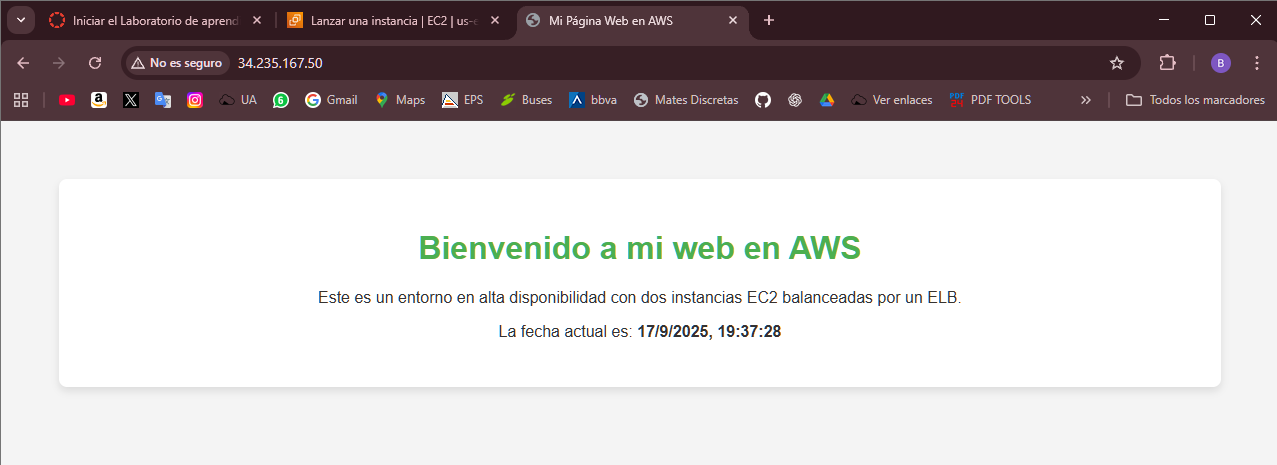
\includegraphics[width=0.95\textwidth]{index.png}
	\caption{http://34.235.167.50/}
	\end{figure}



\newpage


\section{Creación de la segunda instancia}

	Para este apartado debemos de crear una imagen AMI a partir de la instancia base que ya tenemos ejecutando. Esta imagen que usaremos ya tiene instalado httpd, tiene dentro el index.html y el servidor Apache encendido y habilitado. De esta forma no tendremos que conectarnos a ella mediante ssh a no ser que queramos modificar algo.

\subsection{Creación de la AMI}

	Para crear la AMI seleccionamos la instancia de la cual queremos hacer la imagen y le damos a ``Crear imagen'' escribimos un nombre y la guardamos.

	

	\begin{figure}[H]
	\centering
	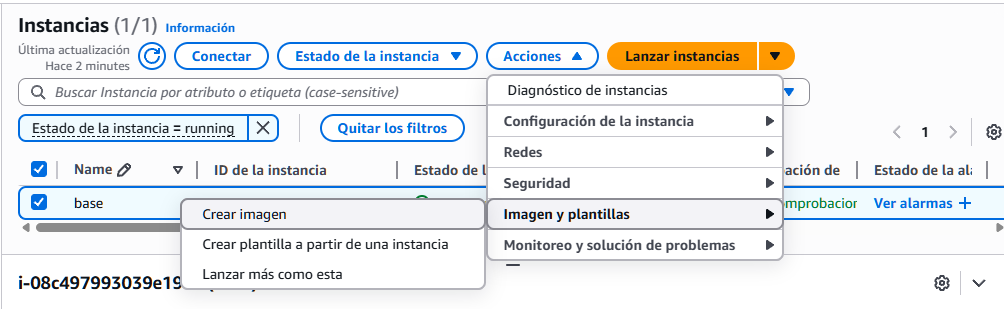
\includegraphics[width=0.95\textwidth]{crear_imagen.png}
	\caption{panel de instancias}
	\end{figure}

\subsection{Instancia a partir de la AMI}
	Una vez que tengamos la AMI debemos de lanzar una instancia nueva a partir de esta para probar su correcto funcionamiento. Esto lo haremos accediendo al menu de ``lanzar instancia'', para esta instancia y en el apartado de 

	
	\begin{figure}[H]
	\centering
	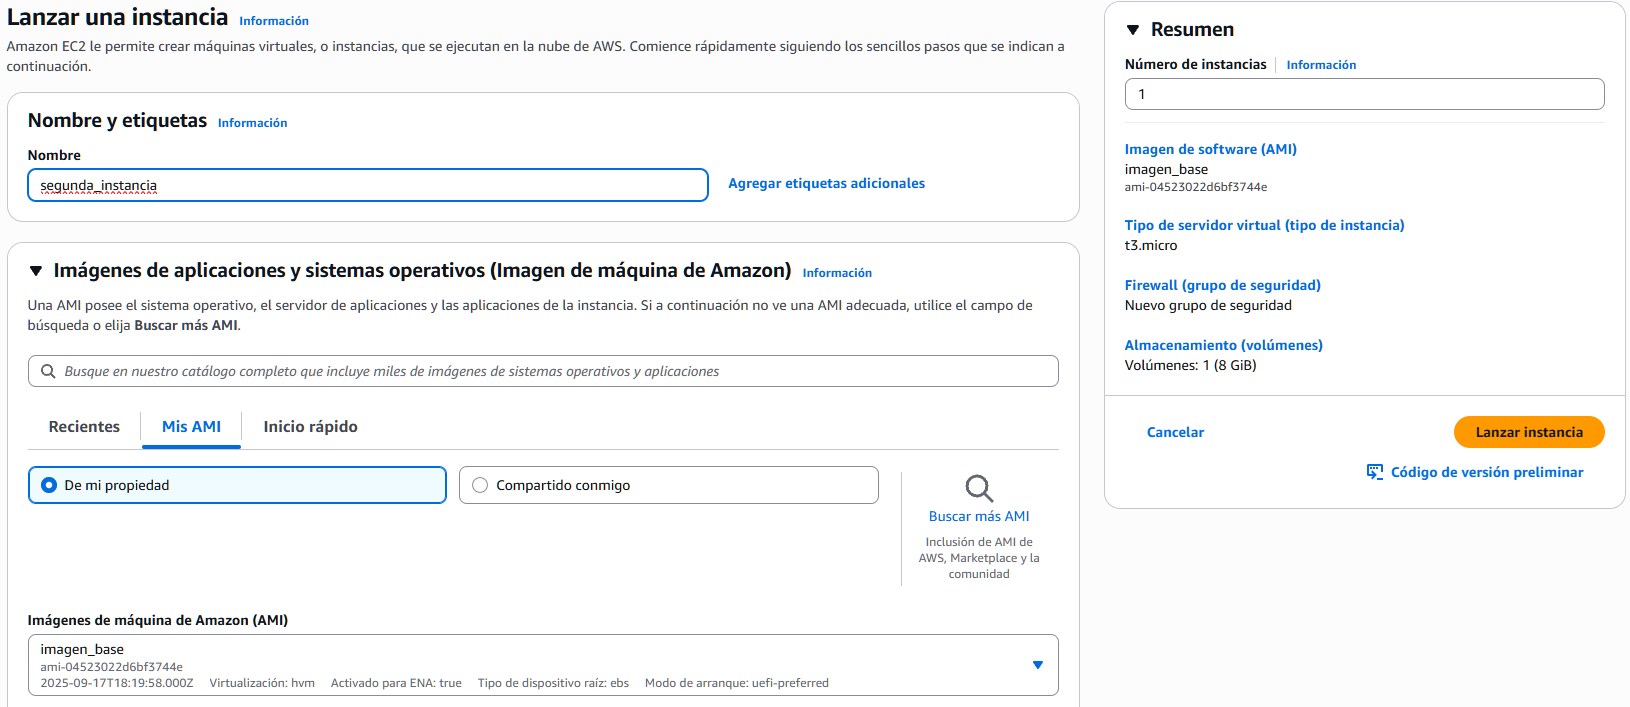
\includegraphics[width=0.95\textwidth]{menu_lanzar_desde_imagen.png}
	\caption{panel de lanzar una instancia}
	\end{figure}

\newpage

\subsection{Acceso Index de la segunda instancia}

	Desde el menu de instancias ya nos aparecerán las dos instancias. Y desde la configuración podremos acceder al ip publico de esta nueva instancia y comprobar si se muestra nuestro index.

	\begin{figure}[H]
	\centering
	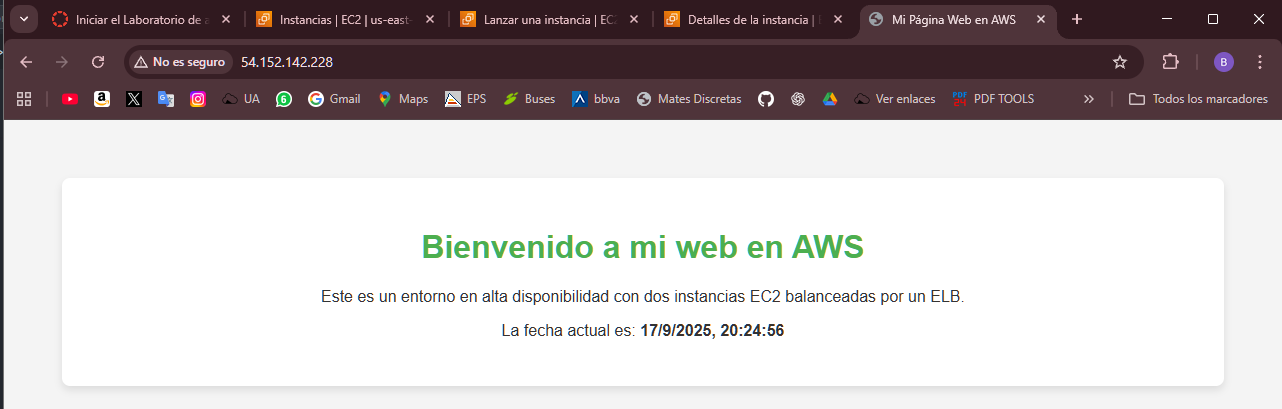
\includegraphics[width=0.95\textwidth]{index2.png}
	\caption{http://54.152.142.228/}
	\end{figure}



	 
\end{document}
